\newpage
\section{Value of Routes}
\subsection{Longer Routes are Overvalued}\label{sec:overvalued}
The reward for owning routes substantially increases for longer routes.
From \cref{table:current_value},
we see that the trains in one- or two-train routes are worth one point
whereas the trains in the six-train routes are worth two and half points.
The ostensible reason for the increasing value per train is that
it takes much more time to collect longer routes than shorter routes.
However in \cref{sec:collecting_cards} we will show the expected 
number of turns to collect $k$ cards of a specific
color is linear in relation to $k$
(rather than polynomial like the current scoring method).

\begin{table}[H]
\renewcommand{\arraystretch}{1.5}
\centering
\begin{tabular}{| c | c | c | c | c | c | c |}
\hline
 Route Length & 1 & 2 & 3 & 4 & 5 & 6\\
 \hline
 Points Scored & 1 & 2 & 4 & 7 & 10 & 15\\
 \hline
 Points per Train & 1 & 1 & $1.\overline{3}$ & 1.75 & 2 & 2.5\\
 \hline
\end{tabular}
\caption{The points scored for building routes by length of route
and per the number of trains.}
\label{table:current_value}
\end{table}

Longer routes are more attractive for players.
First, the reward per train is much higher.
Instead of receiving six points for six one-train routes,
a player can receive 15 points for one six-train route.
Second, players may only buy one route per turn.
It would take a player nine turns--three to collect six cards 
and six to buy six routes--to get six points from one-train routes.
In those same nine turns, a player who spends seven turns collecting
14 cards has the chance to buy two six-train routes
and then get 30 points in their last two turns.
(While it is far from guaranteed that two sets of this player's 14 cards are
six of the same color, the option to choose from five face up cards
on the table makes it more likely that the player has six of the same color.)

The longer route strategy performs even better over many turns.
In an ideal game, a player can collect 46 train cards in 23 turns
and spend eight turns (throughout or at the end) buying all six
six-train routes, one five-train route, and one four-train route.
Because the player has 46 cards, there is a very high likelihood that
they have roughly six cards of each color.
In total, they will have accumulated 107 points and ended the game in 31 turns
where each turn, on average, earns them about three and half points.
The challenge for this strategy is that, unless the player is very lucky,
the two Destination Tickets from the beginning of the game will count
against their score.
Nonetheless, the longer route strategy has remarkable potential.

\subsection{Expected Cards to Build a Route}\label{sec:collecting_cards}
In this section, we find the expected number of cards
$N_k$ we need to see in order to find the $k$ cards of a specific color
needed to build a particular route.
Our argument is that $\E[N_k]$ is better than the
current reward scheme.

Let $C$ be the set of all cards and $k$ be a fixed integer
between 1 and 6, inclusive.
Without loss of generality say we are looking
for blue cards and call this set $B$.
In order to find how long it takes to find $k$ blue cards,
think of our well-shuffled deck as
blue cards separated by non-blue cards.
For example, our deck may have the ordering
\begin{align}
    xxxbxbxxxx...xxbxxx \nonumber
\end{align}
where $x$ is a non-blue card in $C \setminus B$
and $b$ is a blue card in $B$.

Now let $N_k$ be the number of cards until
we see the $k^{th}$ blue card.
Our strategy is to write $N_k$ in terms of
indicator random variables.
Let $I_{k,x}$ be the indicator that takes value 1
if non-blue card $x$ appears before the $k^{th}$ blue card
and 0 otherwise.

The number of cards until the $k^{th}$ blue card
is certainly the number of blue cards $k$
plus the number of non-blue cards before the $k^{th}$ blue.
Written as an equation,
\begin{align}
    N_k = k + \sum_{x \in C \setminus B} I_{k,x}. \nonumber
\end{align}
We are interested in the average number of cards
so we take the expectation of $N_k$ and distribute
over addition via linearity of expectation.
Then
\begin{align} \label{eq:expected_card}
    \E[N_k] = \E[k] + |C \setminus B| \times \E[I_{k,x}].
\end{align}
Since $k$ is fixed, $\E[k]$ is simply $k$.
Since $B$ is a subset of $C$ and both sets are fixed,
$\E[|C \setminus B|]$ is $|C| - |B|$.
Thus we need only find $\E[I_{k,x}]$.

To calculate $\E[I_{k,x}]$, think of the deck as $|B| + 1$ sequences 
of non-blue cards separated by $|B|$ blue cards.
(It is possible for a sequence to be of length zero
in the case that two blue cards are adjacent to each other or
in the case that the first or last card is blue.)
Since we assume the deck is well-shuffled, the non-blue cards
are uniformly distributed across the $|B| + 1$ sequences:
it is as likely for card $x \in C \setminus B$ to be in any one sequence
as any other.

Now think of the indicator $I_{k,x}$ that card $x$ appears
before the $k^{th}$ blue in terms of which of the $|B| + 1$
sequences $x$ resides in.
When looking for only one blue card,
we see that card $x$ appears before the first blue if and only if
$x$ is in the first sequence.
Since $x$ is uniformly distributed across all $|B| + 1$ sequences,
the probability that $x$ appears before the first blue $\p(I_{1,x})$
is $1/(|B| + 1)$.
Similarly, the probability that $x$ appears before the second blue
$\p(I_{2,x})$ is $2/(|B| + 1)$.
By extension, the probability that $x$ appears before the $k^{th}$
$\p(I_{k,x})$ is $k/(|B| + 1)$.

Recall that $I_{k,x}$ takes value 1 if $x$ appears before the 
$k^{th}$ blue and 0 otherwise.
Then, conditioning on $I_{k,x}$, we write its expectation
\begin{align} \label{eq:expected_indicator}
    \E[I_{k,x}] &= 1 \times \p(I_{k,x})
    + 0 \times (1-\p(I_{k,x}) \nonumber \\
    &=\p(I_{k,x}) = \frac{k}{|B| + 1}
\end{align}
Substituting \cref{eq:expected_indicator} in \cref{eq:expected_card},
we have
\begin{align}
    \E[N_k] &= k + |C \setminus B| \times \left(\frac{k}{|B| + 1}\right)
    \nonumber \\
    &= \left(1 + \frac{|C| - |B|}{|B| + 1} \right)k. \nonumber
\end{align}
and, by plugging in the values of $|C|$ and $|B|$,
\begin{align}
    \E[N_k] &= \left(1 + \frac{110 - 12}{12 + 1} \right)k \nonumber \\
    &= \frac{111}{13}k. \nonumber
\end{align}
While  $111/13$ has no obvious units or interpretation,
we have learned that $\E[N_k]$ is proportional to $k$.
That is, the expected number of cards needed to
purchase a route is proportional to the length of the route.

\subsection{Optimal Route Value via Simulations}
We contend that the reward for purchasing a route 
should be related to the effort expended to do so.
Using the number of cards needed to purchase a route 
as a proxy for effort, it is clear from \cref{sec:collecting_cards}
that the reward for a route should be proportional to
its length.
However, we do not know the correct value of the constant $\alpha$
for $\E[N_k] = \alpha k$.

In order to choose a good $\alpha$, we simulate 
\textit{Ticket to Ride} games and track how various
strategies perform.
For each $\alpha$ between 1 and 5 in .2 increments,
we simulate 1000 games where the reward for a route
of length $k$ is $\alpha k$.
The results appear in \cref{fig:points}.

The winning proportions of the Hungry, Path, and One
Step agents are independent of $\alpha$.
However, the Long Route agent--which
depends on the reward from long routes--
performs better with higher values of $\alpha$.
We recommend an $\alpha$ value of 
3.5 because the One Step
and Long Route strategies perform roughly as well at that point.

\begin{figure}[h]
    \centering
    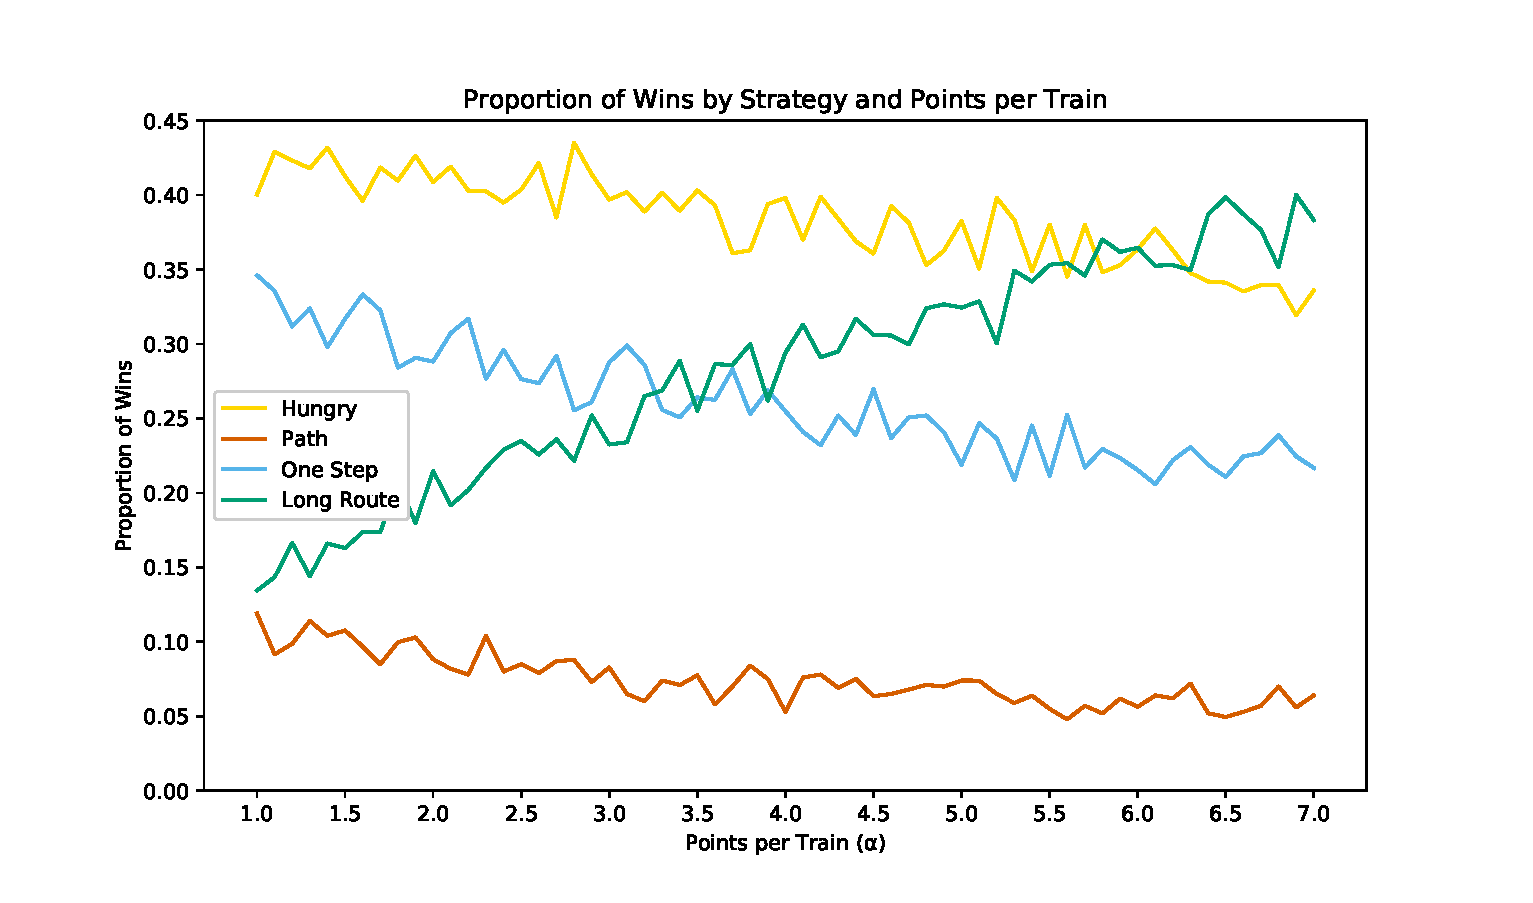
\includegraphics[scale=.65]{figures/points}
    \caption{The proportion of wins of each of the four strategies
    by the number of points earned per train in 1000 games.}
    \label{fig:points}
\end{figure}
